\setmainfont{Noto Serif}
\setsansfont{Noto Sans}
\setmonofont{Noto Sans Mono}
\setstretch{1.35}

\section{Теория кристаллического поля}
1С. Определите расщепление электронных уровней основного терма иона $\text{Ti}^{3+}$ ($3d^1$) в октаэдрическом комплексе, в котором расстояния до всех лигандов одинаковые, а заряд одного из лигандов в два раза меньше, чем заряд остальных пяти.
\par
2С. Определите расщепление электронных уровней основного терма центрального атома металла с электронной конфигурацией $3d^1$ в поле лиганда, представляющего собой окружность радиуса $a$, по которой равномерно распределен заряд $Q$.
\par
3С. Определите расщепление электронных уровней основного терма центрального атома металла с электронной конфигурацией $p^2$ в координационном соединении, имеющем квадратное строение.
\par
4. Определите изменение энергии $3d_{z^2}$ орбитали при удалении двух аксиальных лигандов из комплекса иона $\text{Ti}^{3+}$ ($3d^1$), имеющего строение правильной треугольной бипирамиды.
\par
5. Определите расщепление электронных уровней основного терма иона $\text{Ti}^{2+}$ ($3d^2$) в октаэдрическом комплексе.
\par
6С. Используя теорию поля лигандов качественно опишите электронное строение тетраэдрического аминокомплекса металла с конфигурацией $3d^n$.
\par
7С. Объясните, почему коэффициент экстинкции комплекса цис-$\text{[Co(NH}_3)_4\text{Cl}_2]^+$ заметно больше, чем соответствующего транс-изомера.
\par
8. Сравнить относительную возможность протекания реакций замещения в~октаэдрических комплексах по механизму $S_{N}1$ (переходное состояние – квадратная пирамида) и $S_{N}2$ (переходное состояние – пентагональная бипирамида) для электронных конфигураций центрального металла $d^4$, $d^5$, $d^6$. Рассмотреть случаи сильного и слабого поля.
\par
9С. Как расщепляются термы $^4G_g$ и $^4G_u$ в поле тетраэдра?
\par
10. Как будут расщепляться $p$ орбитали в поле двух точечных зарядов $q_1$ и $q_2$, расположенных на оси $х$ на расстоянии $\pm a$ от начала системы координат?
\par
\begin{wrapfigure}{r}{33mm} %this figure will be at the right
    \centering
    \vspace{-3.8mm}
    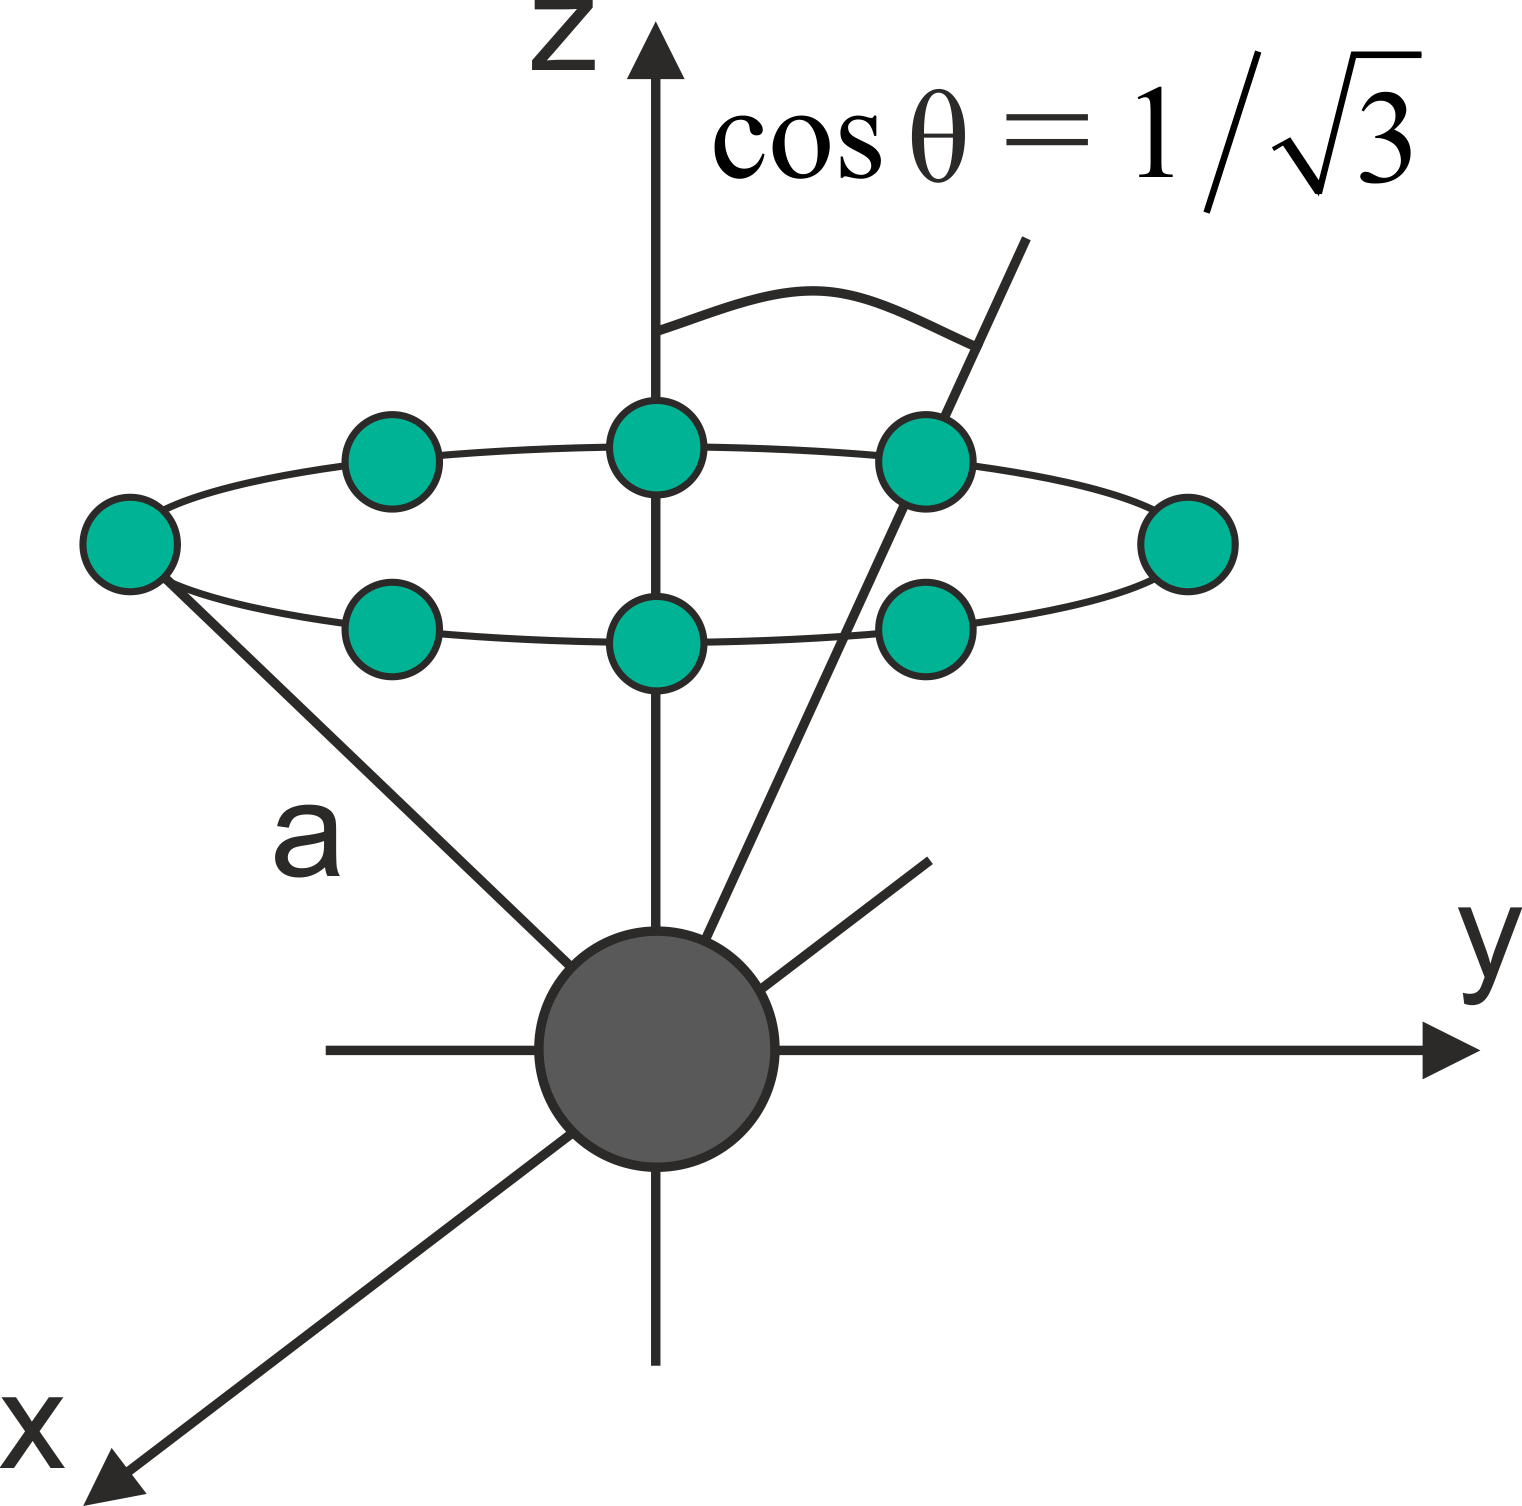
\includegraphics[width=28mm]{images/Fig_2_2_14.png}
    \vspace{-5mm}
\end{wrapfigure}
11К. В структуре цеолитов можно встретить каналы различного размера. Пренебрегая спин-орби-тальным взаимодействием, определите энергию $f_{z^3}$ орбитали иона $\text{Ce}^{3+}$ ($4f^1$), расположенного над восьмичленным кольцом цеолита, как изображено на~рисунке. Лигандные атомы кислорода расположены в~вершинах правильного плоского восьмиугольника. Расстояния от центрального атома до атомов кислорода равны $a$, угол $\theta$ такой, что $\cos\theta=\sqrt{3}/3$. Дополнительные справочные данные приведены ниже.
\\
Некоторые эквивалентные операторы для угловых интегралов с $\textit{Y}_{3m}$:
\vspace{0.1mm}
\begin{equation*}
\begin{aligned}
\widehat L_{60} &= -\frac{1}{2376}\sqrt{\frac{1}{13\pi}}\left( 231\widehat L_z^6-315\widehat L^2\,\widehat L_z^4 +735\widehat L_z^4+105({\widehat L^2})^2\,\widehat L_z^2\,- \right.\\[6pt]
&\quad\qquad\qquad\qquad\ \left. -\,525\widehat L^2\,\widehat L^2_z +294\widehat L^2_z - 5 (\widehat L^2)^3 + 40 (\widehat L^2)^2-60 \widehat L^2 \right);
\\[2pt]
 \widehat L_{64} &= -\frac{1}{1584}\sqrt{\frac{7}{26\pi}}\left( (11\widehat L^2_z - \widehat L^2 -38)(\widehat L^4_++\widehat L^4_-)+(\widehat L^4_++\widehat L^4_-)(11\widehat L^2_z - \widehat L^2 -38) \right); 
\\[6pt]
  \widehat L_{66} &= -\frac{1}{144}\sqrt{\frac{7}{429\pi}}\left(\widehat L^6_++\widehat L^6_-\right); \quad  \widehat L_{44} =\frac{1}{264}\sqrt{\frac{7}{10\pi}} \left( \widehat L_+^4 + \widehat L_-^4  \right);
\\[6pt]
\widehat L_{40} &= \frac{1}{1320}\sqrt{\frac{1}{\pi}}\left( 35\widehat L_z^4-30\widehat L_z^2 \widehat L^2+25\widehat L_z^2-6\widehat L^2+3 (\widehat L^2)^2 \right); 
\\[6pt]
\widehat L_{20} &= -\frac{1}{18}\sqrt{\frac{1}{5\pi}}\left(3\widehat L_z^2-\widehat L^2\right);
\end{aligned}
\end{equation*}
\\
Вид некоторых сферических гармоник $\textit{Y}_{6m}$:
\begin{equation*}
 \begin{aligned}
&\textit{Y}_{60} =\frac{1}{32}\sqrt{\frac{13}{\pi}}\left(231 \cos^6{\theta}-315\cos^4{\theta}+105\cos^2{\theta}-5 \right); 
\\[6pt]
&\textit{Y}_{6\pm4} =\frac{3}{32}\sqrt{\frac{91}{2\pi}} \left( 11\cos^2{\theta}-1\right) \sin^4 {\theta} \, e^{\,\pm4i\phi}; \quad \textit{Y}_{6\pm6}=\frac{1}{64}\sqrt{\frac{3003}{\pi}} \sin^6 {\theta} \, e^{\,\pm6i\phi};\,\,\quad\quad
 \end{aligned}
\end{equation*}
\par
12. Какого типа полосы переноса заряда следует ожидать для координационных соединений $\text{Fe}^{2+}$ и $\text{Fe}^{3+}$ с органическими лигандами?
\par
13. Качественно и количественно определить, как изменится расщепление $d$~орбиталей в поле лигандов квадратной конфигурации, если (1) одну из сторон квадрата повернуть на 90º, (2) каждый лиганд поделить пополам и два получившихся квадрата сдвинуть вверх и вниз, то есть превратить квадрат в~куб. Для обоих случаев нарисовать корреляционные диаграммы.
\par
14. Определить основной терм для случая электронной конфигурации центрального атома $p^2$ в среднем и сильном поле лигандов, которые расположены в вершинах правильного треугольника.
\par
15К. Качественно изобразите корреляционную диаграмму слабое кристаллическое поле $\leftrightarrow$ сильное кристаллическое поле для триплетных термов иона металла с электронной конфигурацией $3d^2$ в тетраэдрическом окружении.
\par